\subsection{Localização}
\label{sec:luz-estruturada}

	Calcular a distância de vários pontos na cena relativa a posição da câmera é uma importante tarefa de sistemas de computação visual~\cite{jain}. Para isso, deve-se obter informações de profundidade das entidades em interesse. Essas informações podem ser obtidas utilizando imagens de intensidade ou de profundidade.

	Uma maneira comum de se obter informações de profundidade de imagens de intensidade é adquirir um par de imagens usando duas câmeras deslocadas entre si por uma distância conhecida. Como alternativa, duas ou mais imagens obtidas de uma câmera em movimento também pode ser utilizadas para calcular informações de profundidade~\cite{jain}. Esse método é conhecido como \textit{Stereo Vision} e necessita ser bem calibrado.  Além disso, os algoritmos que o implementa geralmente são computacionalmente caros e não funcionam em ambiente com baixa condição de iluminação~\cite{fall-detection}.

	Informações de profundidade também podem ser obtidas indiretamente através de imagens de intensidade utilizando sinais na imagem, como sombreamento e textura~\cite{jain}.

	\begin{figure}[hbt]
		\begin{center}
			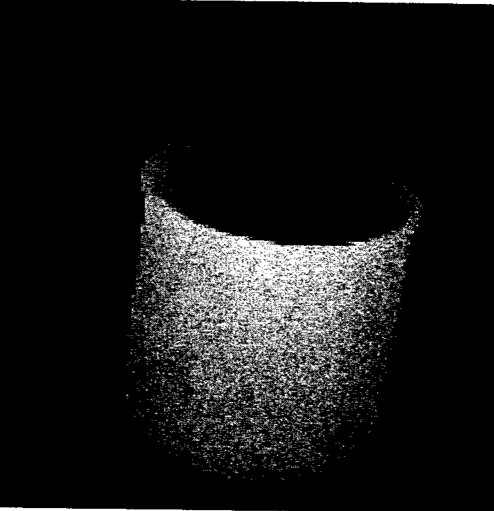
\includegraphics[scale=0.3]{figuras/2.FundamentacaoTeorica/depthimage.png}
		\end{center}
		\caption{Imagem de profundidade de uma caneca de café~\cite{jain}.}
		\label{depthimage}
	\end{figure}

	Em contraste com imagens de intensidade, imagens cujo valor em cada pixel é uma função da distância do ponto correspondente na cena do sensor são chamadas de imagens de profundidade, exemplificada na Figura \ref{depthimage}. Tais imagens podem ser adquiras diretamente utilizando sensores específicos~\cite{jain}. Alguns dos métodos mais conhecidos são:

		\begin{enumerate}
			\item \textbf{Triangulação:} utiliza as propriedades geométricas do triângulo para calcular a localização de entidades. Pode ser dividida em duas subcategorias: lateração e angulação. Lateração computa a posição de uma entidade estimando sua distância de múltiplos ponto de referência. Calcular a posição de uma entidade em duas dimensões requer estimativas de distância de três pontos não colineares como mostrado na Figura \ref{lateration}. Já em três dimensões são necessários quatro pontos não coplanares. Ângulação utiliza ângulos para determinar a distância da entidade. Em geral, ângulação em duas dimensões requer estimativas de dois ângulos e a estimativa da distância entre dois pontos de referência como mostrado na Figura \ref{angulation}~\cite{triangulacao};

			\item \textbf{Tempo de Vôo(\textit{Time of flight} - TOF):} a distância até a entidade é calculada observando a diferença de tempo entre o pulso eletromagnético transmitido e recebido. A informação de profundidade também pode ser obtida através da detecção da diferença de fase entre as ondas transmitidas e as recebidas de um feixe de amplitude modulada~\cite{jain, fall-detection}. Câmeras TOF provêem imagens de profundidade com melhor acurácia em relação ao método de \textit{Stero Vision}, porém são muito caras e pouco acessíveis~\cite{fall-detection};

			\item \textbf{Luz Estruturada (\textit{Structured Light}):} uma imagem de profundidade não pode ser obtida utilizando somente um sensor de vídeo. Porém, adicionando uma textura artificial na cena, como na Figura~\ref{fig:structured-light}, uma imagem de profundidade pode ser recuperada. Esse princípio consiste na projeção de pontos de luz infra-vermelhos na cena e observados por uma câmera infra-vermelha. Trata-se de um método bem mais acessível que o Tempo de Vôo. Porém, é pouco eficiente para estimar a distância dos pontos nas bordas dos objetos, em áreas muito longe do sensor~\cite{fall-detection};
		\end{enumerate}

		\begin{figure}[hbt]
			\begin{center}
				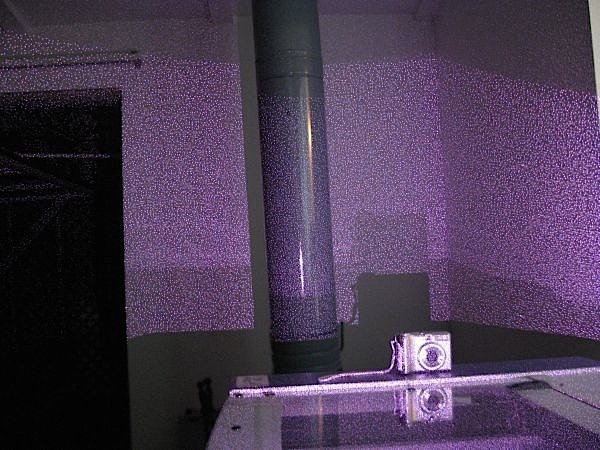
\includegraphics[scale=0.5]{figuras/2.FundamentacaoTeorica/structured-light.jpg}
			\end{center}
			\caption{Exemplo de uma textura artificial adicionada a cena por meio de pontos de luz infra-vermelha utilizando o método Luz Estruturada~\cite{img-strutuctured-light}.}
			\label{fig:structured-light}
		\end{figure}

		\begin{figure}[hbt]
		\begin{center}
			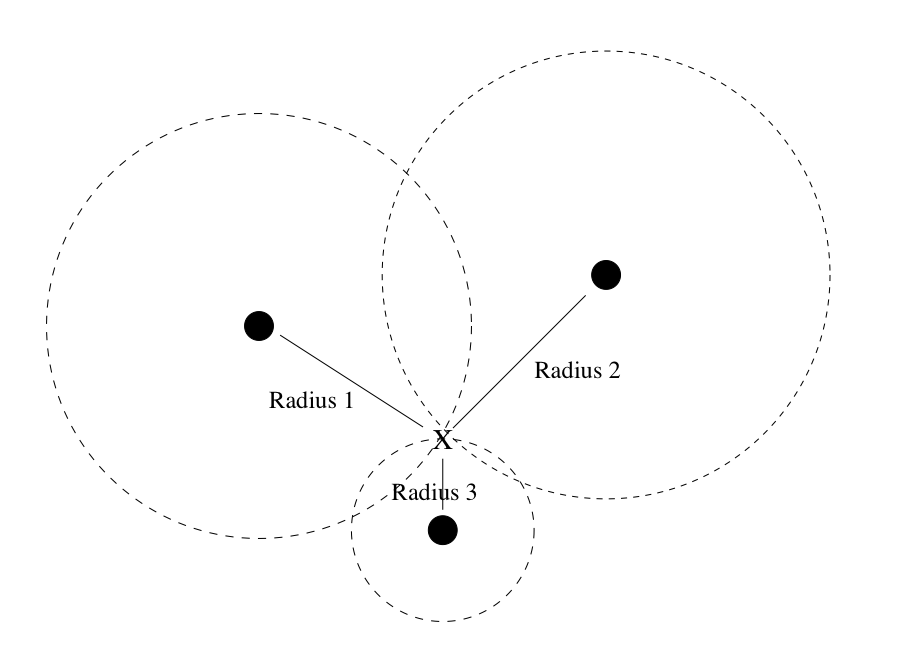
\includegraphics[scale=0.2]{figuras/2.FundamentacaoTeorica/lateration.png}
		\end{center}
		\caption{Determina a distância em duas dimensões utilizando lateração. Requer a distância entre a entidade $\displaystyle X$ e três pontos de referência não colineares~\cite{triangulacao}.}
		\label{lateration}
	\end{figure}

	\begin{figure}[hbt]
		\begin{center}
			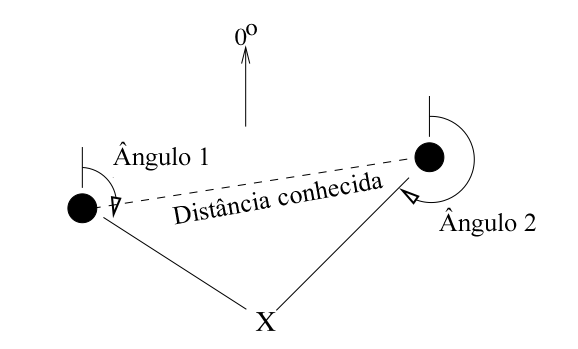
\includegraphics[scale=0.4]{figuras/2.FundamentacaoTeorica/angulation.png}
		\end{center}
		\caption{Exemplo de uma angulação em duas dimensões em que se localiza a entidade $\displaystyle X$ utilizando ângulos relativos a um vetor de referência $\displaystyle 0º$ e a distância entre dois pontos de referência~\cite{triangulacao}.}
		\label{angulation}
	\end{figure}


	Imagens de profundidade são úteis devido a sua especificação explícita de valores de profundidade. Ao mesmo tempo acreditava-se que se a informação de profundidade fosse disponibilizada de maneira explícita, o processamento posterior da imagem seria facilitado. Tornou-se claro que a informação de profundidade ajuda, porém a tarefa básica de interpretação de imagens mantém todas as suas dificuldades~\cite{jain}.

